\section{Installation guide for local development}
First of all you have to install \href{https://www.npmjs.com/}{Npm} and \href{https://git-scm.com/}{Git}. Check if they are working correctly typing in your terminal \shellcmd{node -v}\shellcmd*{npm -v}\shellcmd*{git --version}

After that, if you're using Windows digit \shellcmd{npm install --global --production windows-build-tools} to install Python and other utilities that are necessary to make the demo works.

Download or clone the repository hosted at \url{https://github.com/SOS-SonsOfSwe/Marvin-SoS}.

Install \href{https://metamask.io/}{MetaMask} as an extension for a supported browser.

\noindent Go inside the repository folder (in case you aren't already there) and use npm to install other required programs typing the following commands:
\shellcmd{npm install -g ganache-cli}
\shellcmd*{npm install -g truffle}

Type \shellcmd{npm install}
\label{GanacheDeployment}
Make executable the scripts \emph{startBlockchain.ps1} and \emph{loadProject.ps1} (if you're using an UNIX-like operating system you can type \emph{chmod +x $<$nameOfTheFile$>$}).

Execute the script \emph{startBlockchain.ps1} or otherwise type \textbf{ganache-cli -a 10 -m "candy maple cake sugar pudding cream honey rich smooth crumble sweet treat" -p 9545} to get the same result.

After that open a new terminal in the same folder and execute the script \emph{loadProject.ps1}, otherwise to get the same result you can type the following commands:
\shellcmd{truffle compile}
\shellcmd*{truffle migrate}
\shellcmd*{npm run start}

At this point you will notice that your browser is automatically started and that it visualizes the webpage of \ProjectName{} running at the localhost address. Now you have to connect MetaMask: in your browser click on the MetaMask icon and accept the Privacy Notice and the Terms of use. Then click on \textbf{Main Network} and choose \textbf{Custom RPC}, type in the first form \textbf{http://localhost:9545} as in Figure~\ref{fig:metamask1} and click \textbf{Save}.
\begin{figure}[H]
	\centering
	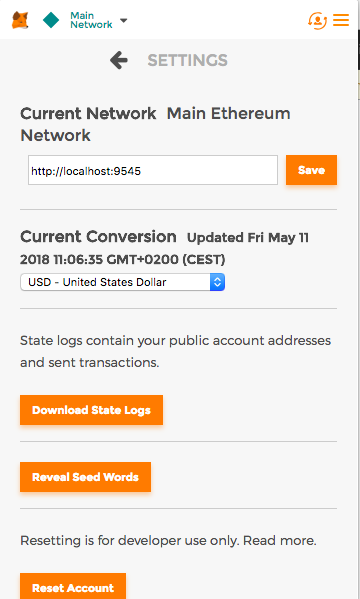
\includegraphics[width=0.35\textwidth]{img/settings.png}
	\caption{Set the RPC typing \textbf{http://localhost:9545}}
	\label{fig:metamask1}
\end{figure}

Now as in Figure~\ref{fig:metamask2a}  click on \textbf{Import Existing DEN} and (as in Figure~\ref{fig:metamask2b}) insert the seed phrase \textbf{candy maple cake sugar pudding cream honey rich smooth crumble sweet treat} and the password that you want to use for the account. Now you're ready to contribute to the development of \project!

\begin{figure}[H]
	\centering
	\begin{subfigure}{0.48\textwidth}
		\centering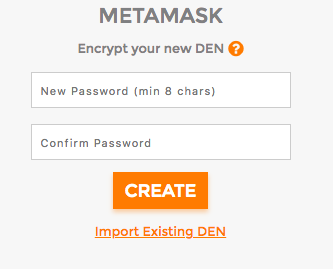
\includegraphics[width=0.65\textwidth]{img/import.png}
		\caption{Click \textbf{Import Existing DEN}}\label{fig:metamask2a}
	\end{subfigure}
	\begin{subfigure}{0.48\textwidth}
		\centering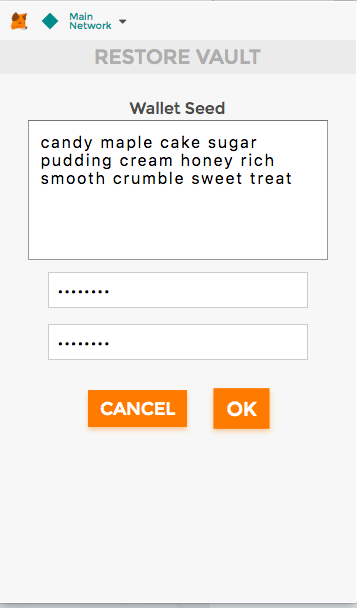
\includegraphics[width=0.65\textwidth]{img/stringPsw.png}
		\caption{Metamask DEN and seed phrase}\label{fig:metamask2b}
	\end{subfigure}
	\caption{main caption}
	\label{fig:metamask2}
\end{figure}
